\documentclass[aspectratio=169]{beamer}

\mode<presentation>
{
  \usetheme{Frankfurt}
  \usecolortheme{crane}
  \usefonttheme{default}
  \setbeamertemplate{navigation symbols}{}
  \setbeamertemplate{caption}[numbered]
}

\usepackage[english]{babel}
\usepackage[T1]{fontenc}
\usepackage[utf8]{inputenc}
\usepackage{booktabs}
\usepackage{amsmath}
\usepackage{array}
\usepackage{graphicx}

\graphicspath{{../reports/figures/}}

\title[Traffic Speed Forecasting on PEMS08]
{Forecasting Average Traffic Speed\\on the PEMS08 Sensor Network}
\subtitle{Near-future and long-term traffic speed forecasting}
\author[Vita Naglič, Matevž Rom, Nace Kovačič]
{Vita Naglič \and Matevž Rom \and Nace Kovačič}
\institute{Artificial Intelligence}
\date{}

\setbeamertemplate{footline}
{
  \leavevmode%
  \hbox{%
  \begin{beamercolorbox}[wd=.42\paperwidth,ht=2.4ex,dp=1.1ex,center]{author in head/foot}%
    \usebeamerfont{author in head/foot}\insertshortauthor{} (Artificial Intelligence)
  \end{beamercolorbox}%
  \begin{beamercolorbox}[wd=.43\paperwidth,ht=2.4ex,dp=1.1ex,center]{title in head/foot}%
    \usebeamerfont{title in head/foot}\insertshorttitle
  \end{beamercolorbox}%
  \begin{beamercolorbox}[wd=.15\paperwidth,ht=2.4ex,dp=1.1ex,center]{date in head/foot}%
    \usebeamerfont{date in head/foot}\insertframenumber{} / \inserttotalframenumber
  \end{beamercolorbox}}%
  \vskip0pt%
}

\newcommand{\missingfigure}[2]{%
  \begin{center}
    \fbox{%
      \begin{minipage}[c][#1][c]{0.88\linewidth}
        \centering
        \textbf{Placeholder}\\[0.5em]
        #2
      \end{minipage}
    }
  \end{center}
}

\begin{document}

\begin{frame}
  \titlepage
\end{frame}

\section{Introduction}

\begin{frame}{Traffic Speed Forecasting as Graph Time Series}
\fontsize{8}{9.6}\selectfont
\begin{columns}[T,totalwidth=\textwidth]
\begin{column}{0.4\textwidth}
\textbf{Task}

Recent sensor history $\rightarrow$ future sensor speed?

\vspace{0.6em}
\textbf{Forecast ranges}

\begin{itemize}
  \item near future: +5 to +60 min
  \item longer term: +1h, +3h, +6h, +12h
\end{itemize}

\vspace{0.6em}
\textbf{Graph view}

\begin{itemize}
  \item node-level regression
  \item sensor time series
  \item neighbour traffic context
\end{itemize}

\vspace{0.4em}
\textbf{Use case:} travel time, congestion warnings, routing
\end{column}
\begin{column}{0.63\textwidth}
\centering
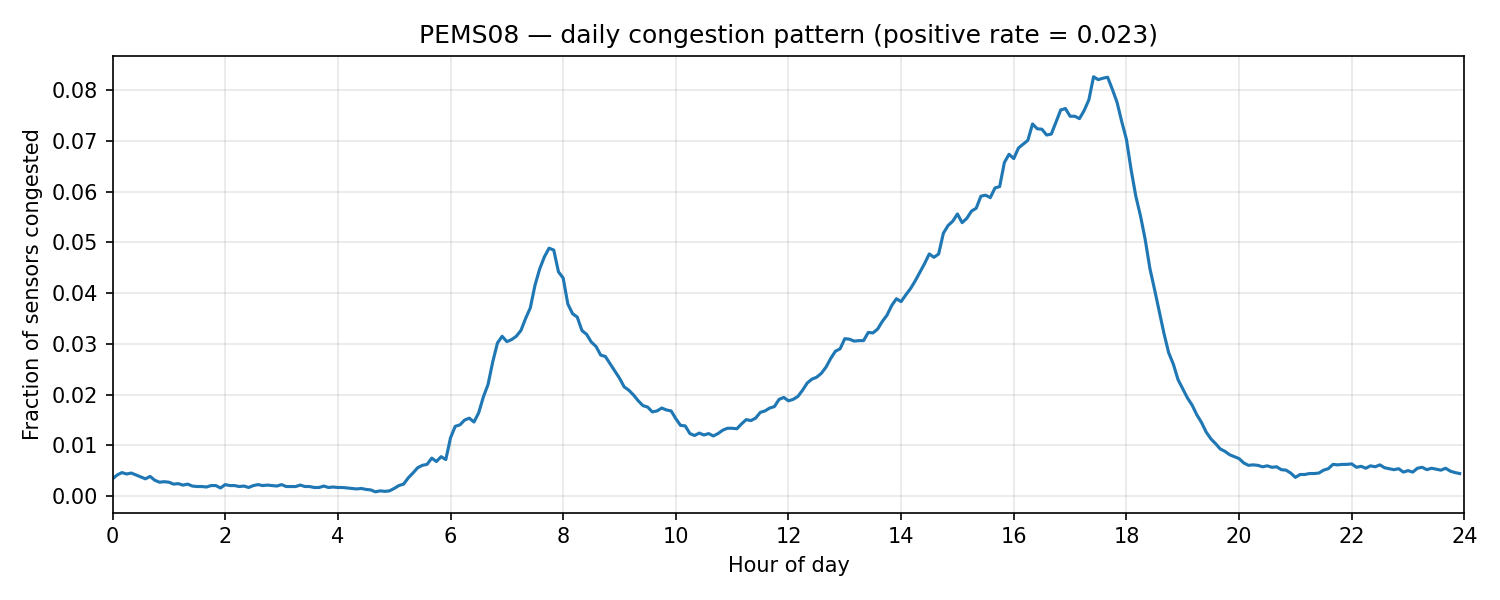
\includegraphics[width=\linewidth,height=0.66\textheight,keepaspectratio]{pems08_daily_congestion.png}
\vspace{-0.9em}

Daily congestion pattern; positive rate: 2.27\%.
\end{column}
\end{columns}
\end{frame}

\section{Dataset}

\begin{frame}{PEMS08: Sparse, Connected Road Graph}
\footnotesize
\begin{columns}[T,totalwidth=\textwidth]
\begin{column}{0.55\textwidth}
\begin{figure}
  \centering
  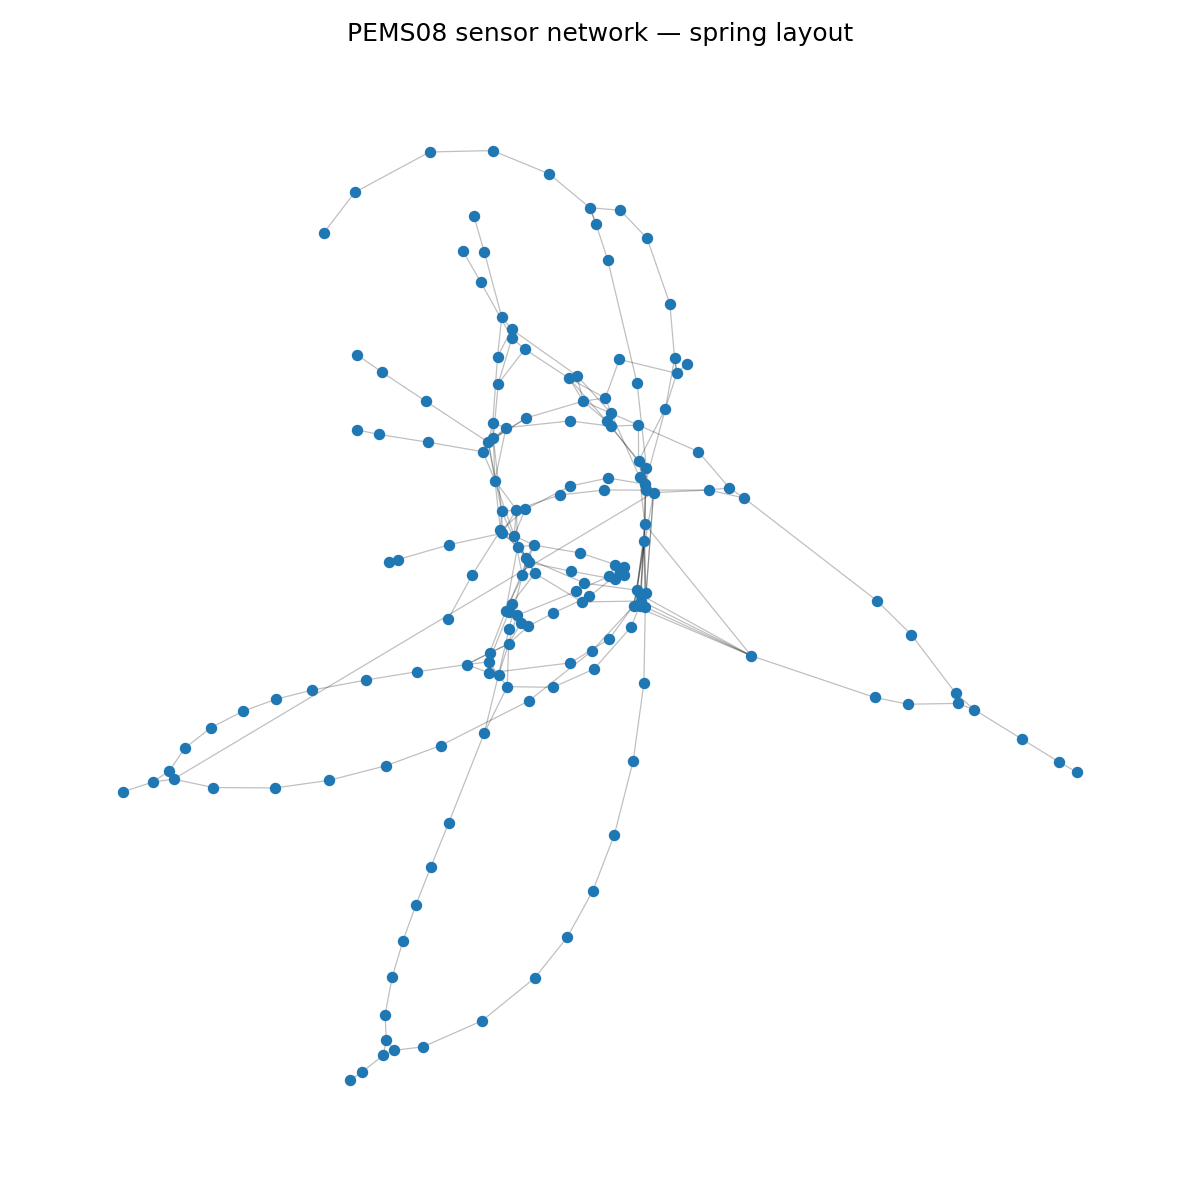
\includegraphics[width=\linewidth,height=0.8\textheight,keepaspectratio]{pems08_network_layout.png}
\end{figure}
\end{column}
\begin{column}{0.40\textwidth}
\textbf{PEMS08 benchmark}

\vspace{0.3em}
\begin{tabular}{@{}ll@{}}
\toprule
sensors & \textbf{170} \\
time steps & \textbf{17,856} \\
resolution & \textbf{5 min} \\
duration & \textbf{62 days} \\
\bottomrule
\end{tabular}

\vspace{0.7em}
\textbf{Road graph facts}
\begin{itemize}
  \item 277 unique directed edges
  \item 1 weakly connected component
  \item avg in/out-degree: 1.63
  \item 16 Louvain communities
\end{itemize}

\vspace{0.5em}
\textbf{Modeling consequence}

Sensor history + nearby-road context
\end{column}
\end{columns}
\end{frame}

\section[NN1]{Neural Network 1: 60 minutes ahead}

\begin{frame}{NN1 -- what goes in and what comes out}
\small
Task: for each sensor, predict its speed one hour from now.

\vspace{0.5em}
Input (what the model sees): the last hour of data from every sensor -- 12 readings, one every 5 minutes.

\vspace{0.5em}
Output (what it predicts): one number per sensor -- the speed in 60 minutes.

\vspace{0.5em}
Each reading gives 10 numbers per sensor:
\begin{itemize}
  \item the 3 measured signals: flow, occupancy, speed;
  \item the time of day and day of week (so it learns rush-hour patterns);
  \item the average of its road-neighbours' signals (what nearby traffic is doing).
\end{itemize}

\vspace{0.5em}
We do not add ``speed X minutes ago'' features -- the last hour is already in the input.
\end{frame}

\begin{frame}{NN1 -- split, normalisation, no leakage}
\small
Temporal (chronological) split: 60\% train / 20\% val / 20\% test.

\begin{itemize}
  \item train = past, test = future $\Rightarrow$ mimics real deployment.
  \item not random k-fold: autocorrelation would leak the future and inflate scores.
\end{itemize}

\vspace{0.6em}
Per-sensor z-score normalisation using training statistics only (features and target);
predictions denormalised back to mph for all metrics.

\vspace{0.6em}
No look-ahead: a gap of $W = 12$ steps is dropped at each split boundary,
so an input window never crosses into another split.
\end{frame}

\begin{frame}{NN1 -- architecture (GCN-GRU) \& training}
\small
Spatial (per time step) -- graph convolution:
\[
H = \operatorname{ReLU}(A X W_{\mathrm{gcn}}), \qquad
A = \alpha A_{\mathrm{fixed}} + (1-\alpha)\tilde{A}, \qquad
\tilde{A} = \operatorname{softmax}(\operatorname{ReLU}(E_1E_2^\top)).
\]

\begin{itemize}
  \item Adaptive adjacency $\tilde{A}$: a learned graph (captures correlations geometry misses).
  \item Residual $H = \operatorname{GCN}(X) + \operatorname{Linear}(X)$: keeps each sensor's own signal.
  \item Temporal: 2-layer GRU over the 12 steps (shared across sensors).
  \item Head: Linear(hidden $\to$ 1) $\Rightarrow$ one speed (60 min). No sigmoid.
  \item Training: Huber loss ($\delta = 1$), Adam (lr $10^{-3}$), early stopping on val MAE,
  seed 42, $\sim$56k params, trained on Apple-Silicon GPU (MPS).
\end{itemize}
\end{frame}

\section[NN2]{Neural Network 2: interval [+5, +60] minutes}

\begin{frame}{NN2 -- predicting the whole interval [+5, +60] min}
\small
Task: for every sensor, predict speed at all 12 steps 5, 10, \ldots, 60 min ahead.

\begin{itemize}
  \item ``Any segment at any near-future time'' -- the data lives on a 5-min grid.
  \item Target grows from [170] to [170, 12] (one value per horizon).
  \item Same 10 features, same 12-step input window as NN1.
  \item Standard benchmark setup (DCRNN, Graph WaveNet report 15/30/60 min jointly).
  \item Both models are kept in the code (flag \texttt{--single-horizon} selects NN1); NN2 is the default.
  \item Neither overwrites the other.
\end{itemize}
\end{frame}

\begin{frame}{NN2 -- what changes vs NN1}
\small
Same spatial GCN + adaptive adjacency + residual, same GRU, same split,
normalisation, loss, training recipe.

\vspace{0.8em}
Only the output head changes:
\[
\operatorname{Linear}(\mathrm{hidden} \to 1)
\quad \Longrightarrow \quad
\operatorname{Linear}(\mathrm{hidden} \to 12)
\]

\vspace{0.4em}
Output shape per sample: [N] $\Rightarrow$ [N, 12]; Huber loss summed over all 12 horizons.

\vspace{0.8em}
Predicting all horizons jointly acts as multi-task regularisation (one model, full curve).

\vspace{0.8em}
Cost: $\sim$60k params (vs $\sim$56k) -- essentially free.
\end{frame}

\section[NN3]{Neural Network 3: long-term horizons}

\begin{frame}{NN3: Later-Today Speed Forecasting}
\footnotesize
\textbf{Goal:} from immediate traffic control to later-today planning

\vspace{0.5em}
\begin{columns}[T,totalwidth=\textwidth]
\begin{column}{0.48\textwidth}
\textbf{Prediction horizons}

\vspace{0.3em}
\begin{center}
\renewcommand{\arraystretch}{1.25}
\begin{tabular}{@{}cccc@{}}
\toprule
\textbf{+1h} & \textbf{+3h} & \textbf{+6h} & \textbf{+12h} \\
12 steps & 36 steps & 72 steps & 144 steps \\
\bottomrule
\end{tabular}
\end{center}

\vspace{0.5em}
\textbf{Target}

\begin{itemize}
  \item speed per sensor
  \item 4 horizons jointly
\end{itemize}
\end{column}
\begin{column}{0.47\textwidth}
\textbf{Leakage-safe inputs}
\begin{itemize}
  \item flow, occupancy, speed at $t$
  \item speed lags: 3h, 6h, 12h, 1d, 2d, 7d
  \item current + target calendar time
\end{itemize}

\vspace{0.4em}
\textbf{Built dataset}
\begin{tabular}{@{}ll@{}}
$X$ & $(15696, 170, 29)$ \\
$y$ & $(15696, 170, 4)$ \\
train / val / test & 9417 / 3139 / 3140 \\
\end{tabular}
\end{column}
\end{columns}

\vspace{0.35em}
\centering
\textbf{No future traffic measurements as inputs}
\end{frame}

\begin{frame}{NN3: Shared-Sensor GRU}
\small
\begin{center}
\large
2 hours of features $\rightarrow$ shared GRU $\rightarrow$ +1h, +3h, +6h, +12h speeds
\end{center}

\vspace{0.4em}
\begin{columns}[T,totalwidth=\textwidth]
\begin{column}{0.48\textwidth}
\textbf{Why this architecture}
\begin{itemize}
  \item small, stable model
  \item temporal patterns shared across sensors
  \item all long horizons in one pass
\end{itemize}
\end{column}
\begin{column}{0.47\textwidth}
\textbf{Best run}
\begin{itemize}
  \item input window: 24 steps = 2 hours
  \item hidden size: 64
  \item GRU layers: 2
  \item dropout: 0.2
  \item parameters: 43,460
  \item loss: Smooth L1 / Huber
  \item device: CUDA GPU
\end{itemize}
\end{column}
\end{columns}

\vspace{0.6em}
\centering
\textbf{Train-only normalisation; metrics in mph}
\end{frame}

\section{Results}

\begin{frame}{Results -- NN1 vs NN2 vs baselines}
\small
\begin{center}
\renewcommand{\arraystretch}{1.18}
\setlength{\tabcolsep}{0.85em}
\begin{tabular}{@{}lccc@{}}
\toprule
Model (test set) & MAE & RMSE & MAPE \\
\midrule
Persistence (avg over 5--60 min) & 1.6133 & 3.7811 & 3.08\% \\
Persistence (60 min only) & 2.1403 & 4.9692 & 4.21\% \\
\addlinespace
NN1 -- single-horizon (60 min) & 1.7979 & 4.4583 & 4.13\% \\
NN2 -- multi-horizon (60 min) & 1.7677 & 4.2927 & 3.98\% \\
NN2 -- multi-horizon (avg) & 1.4897 & 3.6037 & 3.23\% \\
\bottomrule
\end{tabular}
\end{center}

\vspace{0.7em}
At 60 min, NN2 matches/beats NN1 while also covering all shorter horizons.

\vspace{0.5em}
NN2 beats the average persistence by +7.7\% -- and that average is hard (see next slide).
\end{frame}

\begin{frame}{Results -- the crossover (per-horizon MAE)}
\small
\begin{columns}[T,totalwidth=\textwidth]
\begin{column}{0.58\textwidth}
\missingfigure{0.55\textheight}{Per-horizon MAE crossover plot\\Persistence vs. NN2}
\end{column}
\begin{column}{0.37\textwidth}
\textbf{Key finding}

\vspace{0.6em}
Persistence is near-perfect short-term (speed barely changes in 5 min).

\vspace{0.6em}
The model overtakes at $\sim$20 min and the gap grows: +17.4\% at 60 min.

\vspace{0.6em}
$\Rightarrow$ judge models per horizon, not by a single average.
\end{column}
\end{columns}
\end{frame}

\begin{frame}{Results -- ablation (each component helps)}
\small
\missingfigure{0.48\textheight}{Ablation figure\\Fixed graph vs. adaptive adjacency vs. residual}

\vspace{0.6em}
Fixed-graph base is weakest; + adaptive adjacency and + residual each lower MAE.

\vspace{0.5em}
Same trend for NN1 and NN2 -- the gains come from architecture, not scale.
\end{frame}

\begin{frame}{NN3 Result: Lower MAE Across Horizons}
\footnotesize
\begin{columns}[T,totalwidth=\textwidth]
\begin{column}{0.61\textwidth}
  \begin{figure}
    \centering
    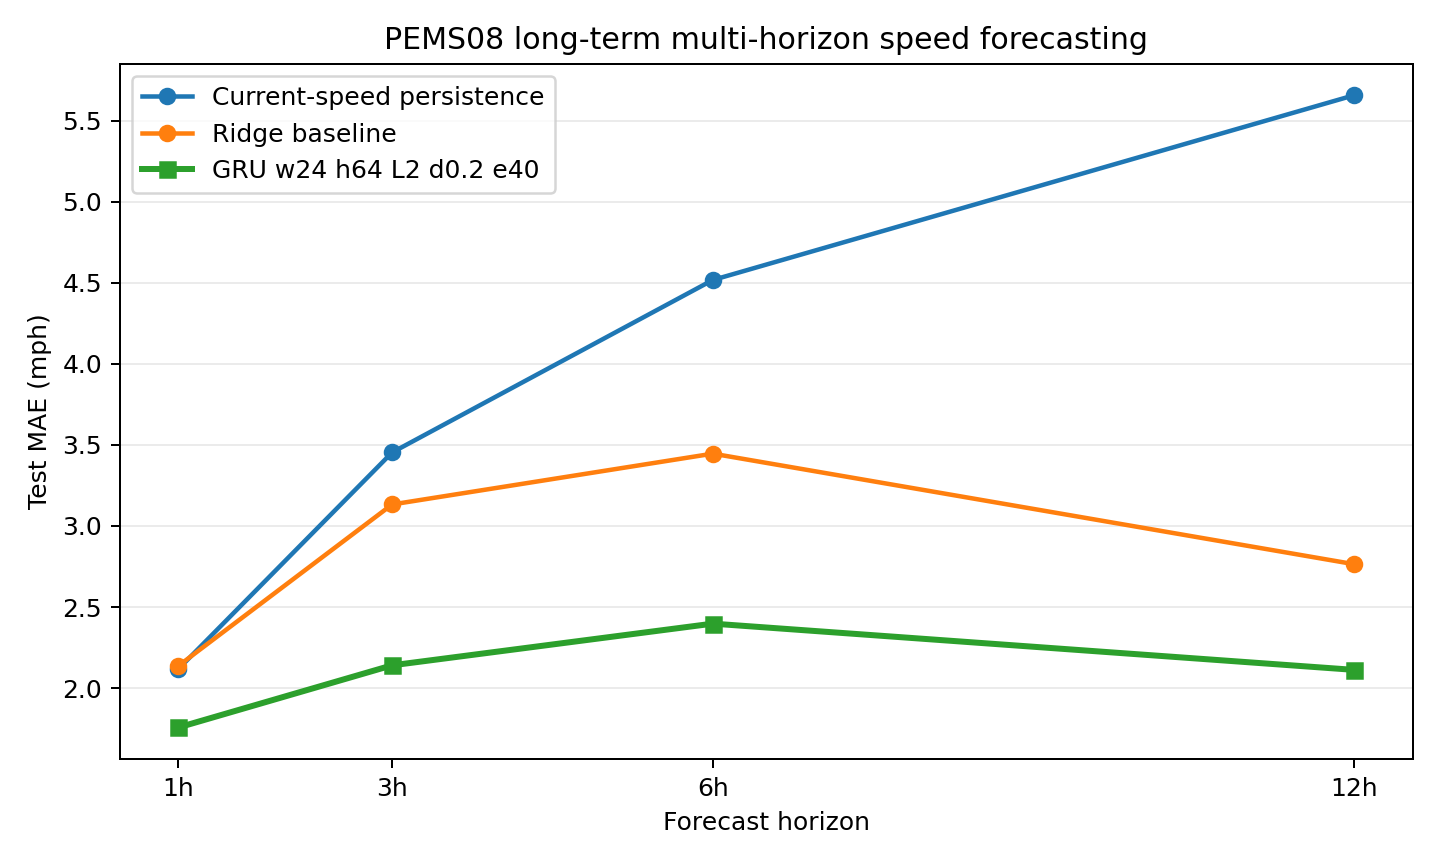
\includegraphics[width=\linewidth,height=0.61\textheight,keepaspectratio]{pems08_longterm_multi_horizon_mae.png}
  \end{figure}
\end{column}
\begin{column}{0.35\textwidth}
\textbf{Best GRU}

\vspace{0.2em}
\Large Avg MAE: \textbf{2.1015}

\vspace{0.6em}
\footnotesize
\textbf{Best baseline: ridge}

\begin{itemize}
  \item ridge avg MAE: 2.8699
  \item GRU improvement: 26.8\%
  \item +6h improves by 1.0489 mph
\end{itemize}

\vspace{0.5em}
\textbf{Interpretation}

\begin{itemize}
  \item hardest horizon: +6h
  \item +12h helped by daily periodicity
\end{itemize}
\end{column}
\end{columns}
\end{frame}

\begin{frame}{Takeaways}
\large
\begin{itemize}
  \item PEMS08: graph time-series forecasting
  \item short horizons: immediate traffic dynamics
  \item NN3: later-today horizons (+1h, +3h, +6h, +12h)
  \item chronological splits + leakage checks
  \item best long-horizon GRU: lowest MAE at every horizon
\end{itemize}
\end{frame}

\end{document}
